%%%%%%%%%%%%%%%%%%%%%%%%%%%%%%%%%%%%%%%%%%%%%%%%%%%%%%%%%%%%%%%%%%%%%%
% How to use writeLaTeX: 
%
% You edit the source code here on the left, and the preview on the
% right shows you the result within a few seconds.
%
% Bookmark this page and share the URL with your co-authors. They can
% edit at the same time!
%
% You can upload figures, bibliographies, custom classes and
% styles using the files menu.
%
%%%%%%%%%%%%%%%%%%%%%%%%%%%%%%%%%%%%%%%%%%%%%%%%%%%%%%%%%%%%%%%%%%%%%%

\documentclass[12pt]{article}

\usepackage{sbc-template}

\usepackage{graphicx,url}

%\usepackage[brazil]{babel}   
\usepackage[utf8]{inputenc}  

     
\sloppy

\title{Ontologias para saúde Mental}

\author{Gustavo L. Schroeder\inst{1}, Leonardo S. Paula\inst{1}}


\address{Universidade do Vale do Rio dos Sinos (UNISINOS)\\
  São Leopoldo -- RS -- Brasil
  \email{AJUSTAR, leonardopaula@gmail.com}
}

\begin{document} 

\maketitle

\begin{abstract}
  
\end{abstract}
     
\begin{resumo} 
  
\end{resumo}


\section{Introdução}

Uma ontologia consiste na especificação formal de uma série de conceitos de um domínio e a relação entre eles \cite{GRUBER1993199}. Segundo \cite{Noy01ontologydevelopment}, diversas são as razões para se criar uma ontologia. Dentre elas: permitir o reuso de um domínio de conhecimento; para analisar um determinado domínio; para compartilhar o entendimento comum de estruturas de informação entre pessoas ou agentes de software. 

%- área de saúde mental; \\
%- porque estamos criando uma ontologia para isso; \\
%- falar da estrutura do artigo: 

\section{Ontologia Base} \label{sec:baseOntology}

Ao se deparar com a definição de um projeto, se torna necessário a formulação de uma série de conceitos e a forma com que estes se relacionam.
Considerando que muitos itens acabam sendo similares para múltiplos conextos, a reutilização além de útil passa a ser recomendável.[Fundamentar]
Sendo assim, foi elaborada uma ontologia para ser utilizada como base e posteriormente expandida, focada nos conceitos fundamentais do acompanhento ubíquo de pessoas com alguma dificuldade ou comorbidade no âmbito psicológico.

A elaboração desta ontologia de base seguiu a abordagem topdown, onde as características abstratas do modelo foram sendo elicitadas e posteriormente expandidas para objetos concretos. Para construção do modelo foi utilizada a ferramenta Protegè.

Nas próximas subseções serão descritas as principais classes relacionadas ao nó raiz (Thing), sua descrição, propriedades e relacionamentos.

\subsection{Class User} \label{sec:userClass}
Consiste na abstração de uma pessoa que interage com o modelo, possuíndo \textit{"Person"} como subclasse, sendo esta a materialização do ente que interage com o sistema e agrega informações como nome e idade.
Esta estrutura permite a expansão para outras figuras da classe \textit{Person}, como médicos e psicólogos, que possam vir a atuar no modelo e se relacionar com o usuário.

\subsection{Class Place} \label{sec:}
Representa o local semântico para a pessoa, representando muito mais do que as coordenadas geográficas, mas sim em um local com significado para a entidade. A classe place é utilizada com a finalidade de correlacionar os índices de saúde mental com as localizações semânticas, estabelecendo uma relação entre a presença de desordens e os lugares que o paciente frequenta.
Está relacionado diretamente a entidade \textit{Location}, filha da classe principal \textit{Context}, que por sua compreende coordenadas geográficas incluindo a latitude, longitude e altitude no momento em que um determinado contexto foi obtido;

\subsection{Class Context}

Responsável pela representação das informações que indicam o contexto em que o usuário se encontra em determinada janela de tempo, esta classe é subdividida em \textit{DailyContext} e \textit{PhysiologicalContext}.

Com estes dados agrupados em momentos no decorrer do tempo, formam-se contextos \cite{dey2001conceptual} que são persistídos numa base de dados, formando históricos de contextos.

\begin{itemize}
    \item \textbf{PhysiologicalContext}
    \begin{itemize}
    \item Agrega informações de natureza fisiológica da pessoa, indicando a qualidade do sono \textit{Sleeping} represetado por pontos em uma escala 0-100, a saturação de oxigêncio no sangue (\textit{Oximetry}), a variabilidade da frenquência cardíaca (\textit{HeartRateVariability}) e a frequência cardíaca (\textit{HeartRate});
    \end{itemize}
    
    \item \textbf{DailyContext}
    \begin{itemize}
    \item Relaciona informações de aspecto ordinário, como data e hora (\textit{DateTime}) que são essenciais para criação uma janela temporal e a etapa do dia (\textit{DayShift}); a atividade em que a pessoa está envolvida (\textit{Activity}), juntamente com a localização geográfica (\textit{Location}) e a quantidade de passos dados \textit{(Steps)};
    \end{itemize}
\end{itemize}

\subsection{Class MentalDisorder}
Criada com o intuito de servir como base para desordens mentais. Representa os problemas mentais que o usuário pode sofrer, permitindo a expansão para novas comorbidades mentais. Podendo ao ser expandida se relacionar com outras entidades para identificar problemas mentais específicos.

\section{Expansões}\label{sec:figs}

Explicar as duas ontologias extendidas;

\subsection{Digital Dependency}
Esta expansão da ontologia descreve o uso não saudável de dispositivos eletrônicos e sua relação com problemas de saúde mental e doenças, usando o histórico de contexto para identificar essas doenças.

\subsubsection{DeviceContext}
    \begin{itemize}
    \item \textbf{SmartphoneAppUse}:
    Esta entidade tem por objetivo agregar informações sobre quais aplicativos o usuário está usando em um dado momento podendo utilizar informações de outras entidades como \emph{DateTime}  para formar históricos de contextos.
    \item \textbf{SmartphoneScreenStatus}:
     Esta entidade tem por objetivo agregar informações sobre qual o status corrente da tela do smartphone (ligada/desligada), podendo ser relacionado com outras entidades para prever contextos e problemas mentais.
    \item \textbf{VideoGameStatus}:
    Esta entidade tem por objetivo agregar informações sobre qual o status corrente do console de jogos do usuário, podendo ser relacionado com outras entidades para prever contextos e problemas mentais.
    \item \textbf{WebBrowserHistory}:
    Esta entidade tem por objetivo agregar informações sobre a frequência e quais sites o usuário utiliza seu navegador, podendo ser relacionado com outras entidades para prever contextos e problemas mentais. Um estudo anterior sugeriu que a análise do histórico de navegação na Web poderia ajudar a prever o estado de saúde mental com uma faixa de precisão de 77,78 \% a 100\% \cite{nie2012predicting}.
    \item \textbf{NotificationStatus}:
    Esta entidade tem por objetivo agregar informações sobre qual o status das notificações do smartphone, podendo ser relacionado com outras entidades para prever contextos e problemas mentais.
    \end{itemize}

\subsubsection{MentalDisorder}
    \begin{itemize}
    \item \textbf{Anxiety}
        \begin{itemize}
        \item \textbf{SocialAnxiety}
        \end{itemize}
    \item \textbf{Depression}
    \item \textbf{MentalDistress}
    \item \textbf{Stress}
    \end{itemize}

\subsubsection {TechnologyAddiction}
    \begin{itemize}
    \item \textbf{InternetAddiction}
    \item \textbf{SmartphoneAddiction}
    \item \textbf{SocialMediaAddiction}
    \item \textbf{VideoGameAddiction}
    \end{itemize}
    
\cite{samaha2016relationships} mostraram a existência de uma relação positiva entre dependência de smartphone e estresse, enquanto \cite{alhassan2018relationship} alertam que a correlação positiva entre o vício em smartphones e a depressão é alarmante. \cite{saikia2019internet} mostram uma associação significativa entre o vício em Internet e depressão, ansiedade e estresse. Frequentemente, há um ciclo vicioso de depressão, resultando em vício em Internet, que gera ainda mais depressão. \cite{dhir2018online}  demonstraram que a fadiga de mídias sociais pode levar à depressão e à ansiedade e \cite{wang2019association} nos trazem a relação do vício em jogos para celular com depressão, ansiedade social e solidão.

\subsection{Expandida 2}
Ontologia do Leonardo.

%\begin{figure}[ht]
%\centering
%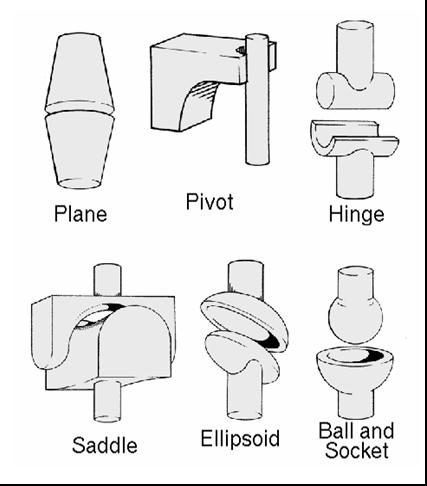
\includegraphics[width=.3\textwidth]{fig2.jpg}
%\caption{This figure is an example of a figure caption taking more than %one
  %line and justified considering margins mentioned in %Section~\ref{sec:figs}.}
%\label{fig:exampleFig2}
%\end{figure}

%\begin{table}[ht]
%\centering
%\caption{Variables to be considered on the evaluation of interaction
  %techniques}
%\label{tab:exTable1}
%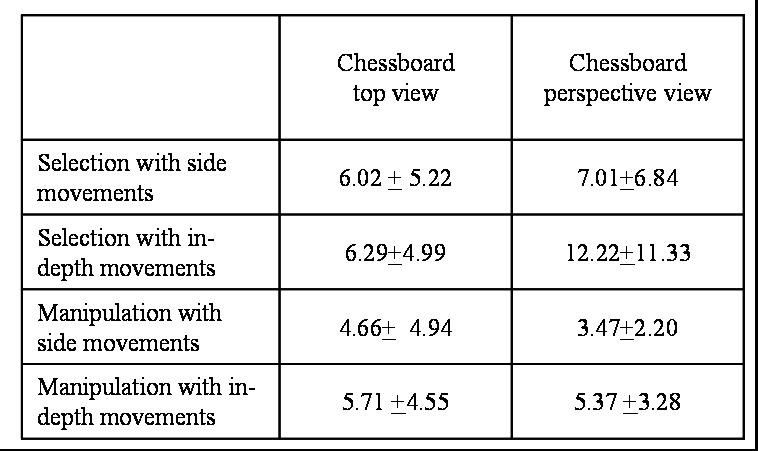
\includegraphics[width=.7\textwidth]{table.jpg}
%\end{table}

\bibliographystyle{sbc}
\bibliography{sbc-template}

\end{document}
